\chapter{Introduction to Plotting}

\section{Introduction}
This exercise will introduce calculations and plotting techniques using
numpy arrays within Scientific Python.

\section{Plotting discrete data and continuous functions}

\begin{figure}[htbp]
\begin{center}
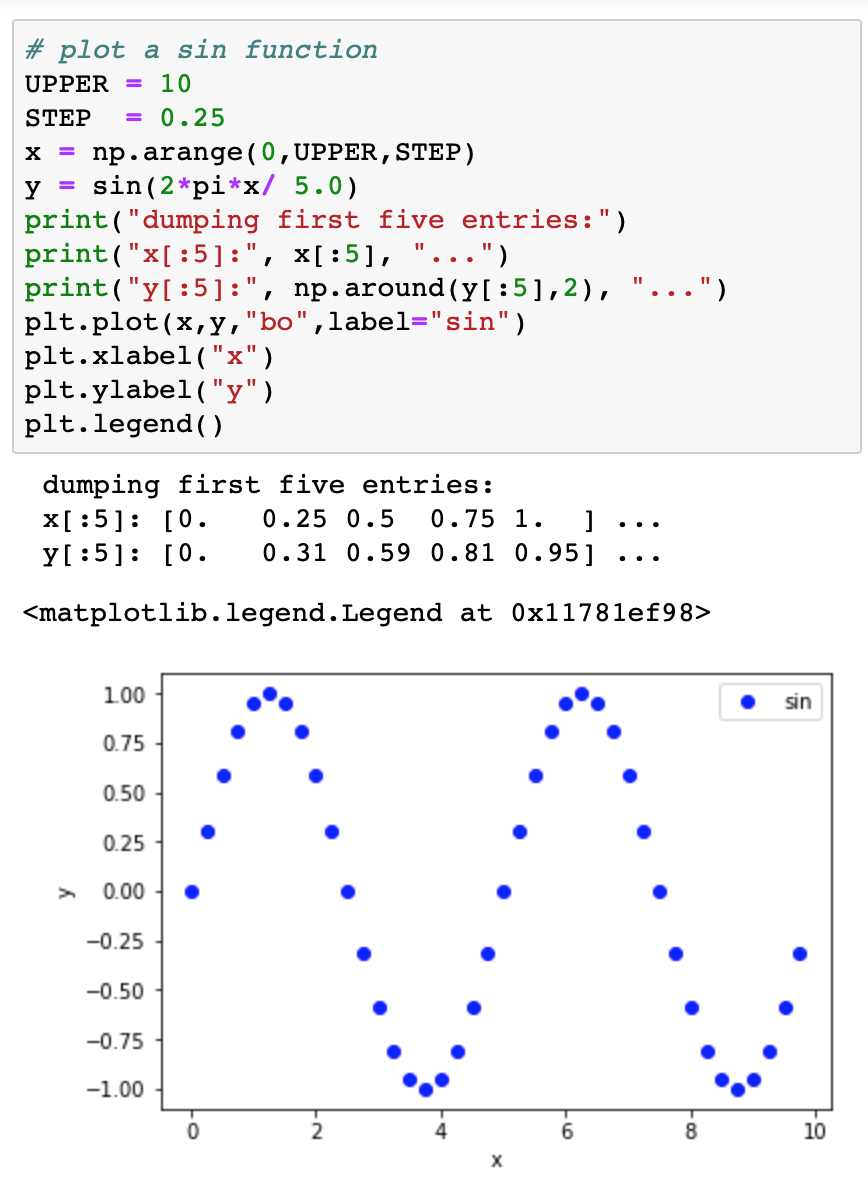
\includegraphics[width=0.65\textwidth]{figs//plotting/plotting.png} 
\caption{Circuit for verifying Ohm's law as a (a) circuit diagram, and (b) implemented using your lab equipment.}
\label{fig:plotsin}
\end{center}
\end{figure}

Consider the Jupyter notebook example in Fig.~\ref{fig:plotsin} which
plots a sine function sampled at discrete values.  Note the following
key features, which you will use repeatedly today and in future labs:
\begin{itemize}
\item Use of global variables {\tt UPPER} and {\tt STEP} at the top of
  the snippet, allowing for easy adjustment of parameters that affect
  the plot.
\item Use of {\tt np.arange} to define an array of x values.
\item Creation of the array y, defined by $y = \sin(2\pi x / 5)$ for each value of x.  One of the great joys of using numpy is the ability to avoid getting bogged down with explicit for loops.
\item Use of slicing techniques {\tt x[:5]} to show only the first five entries for debugging.  
\item Plotting the arrays of $x$ and $y$ values with {\tt plt.plot}  using the {\tt "bo"} option for blue circles.
\item Defining appropriate axis labels with {\tt plt.xlabel} and {\tt plt.xlabel}. 
\item Creation of a legend using the {\tt label} option to {\tt plt.plot} and the {plot.legend()} command.
\end{itemize}
Notice that even in this simple example, I've added some intermediate
feedback from my code in the form of the screen dumps of the first few
values of $x$ and $y$.  It's a common pitfall to try and rush ahead to
the final product when programming.  But it is much faster and
reliable to break your task into small steps, and establish feedback
at each small step.  To plot a continuous function with Scientific
Python, you will still use discrete data but:

\begin{itemize}
 \item Use much finer binning of the $x$-axis variable to draw a smooth curve. 
 \item Use the line option {\tt "-"} or dashed line {\tt "--"} instead of points with {\tt "o"}. 
\end{itemize} 

\noindent
{\bf Plot 1:}  Plot the quadratic function $y = x^2$ with the following requirements:
\begin{itemize}
 \item Plot in the range $x = [0,20)$.
 \item Plot discrete samples with a step size of $2$ using blue circles.
 \item On the same axis, plot the corresponding smooth function using a red solid line.
 \item Add appropriate axis labels. 
 \item Add a legend for the ``discrete'' and the ``smooth''  function.
\end{itemize}

\section{Multivariate analysis using boolean masks}
\begin{figure}[htbp]
\begin{center}
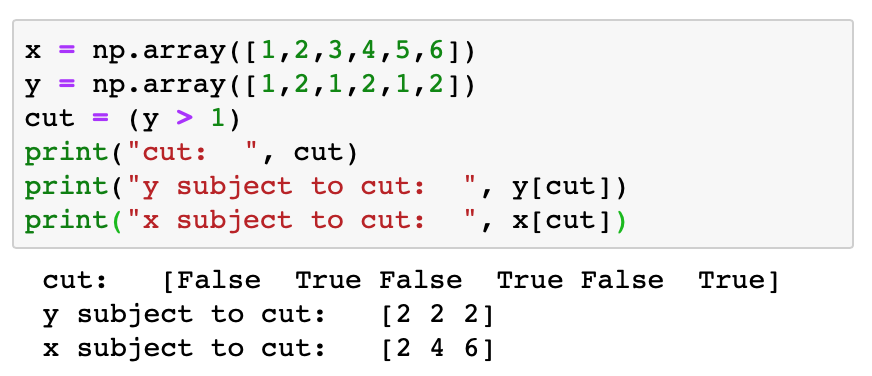
\includegraphics[width=0.65\textwidth]{figs//plotting/booleanmasks.png} 
\caption{Using boolean masks to cut on variable $y$.}
\label{fig:booleanmasks}
\end{center}
\end{figure}

A powerful technique in Scientific Python for performing analysis involving multiple variables uses boolean masks as shown in Fig.~\ref{fig:booleanmasks}.  In the example:
\begin{itemize}
\item Two numpy arrays $x$ and $y$ {\tt of the same length} are defined to contain the collected data.
\item The cut defined by $y > 1$ is a boolean array of the same length as $x$ and $y$ which is true at indices where the condition is met and false where it is not.
\item The subset of the entire $y$ array defined by {\tt y[cut]} consists only of those entries of $y$ for which the condition $y>1$ is met.
\item The subset of the entire $x$ array defined by {\tt x[cut]} consists only of those entries of $x$ for which the condition $y>1$ is met for the corresponding y value.
\end{itemize}
The last item shows the real power of this technique, one can look at one variable subject to constraints on another variable.

\begin{table}
\caption{Sample data for a voltage measurement subject to high frequency noise.}
\label{tbl:hfnoiseeg}
\begin{center}
\begin{tabular}{lll}
$t~(\rm s)$ & $v~(\rm V)$ & $n$ \\
0.4  & 0.25  &  2.8 \\
1.1  & 2.37  &  7.3 \\
1.4  & 1.69  &  9.7 \\
1.9  & 0.93  &  1.3 \\
2.5  & -1.0  &  6.2 \\
3.0  & 0.95  &  4.8 \\
3.4  & 1.22  &  6.9 \\
4.1  & 0.54  &  4.0 \\
4.4  & 0.37  &  1.9 \\
4.8  & 0.13  &  4.0 \\
5.5  & -2.04  &  9.5 \\
6.2  & -2.06  &  8.7 \\
6.5  & -0.81  &  2.3 \\
7.0  & -0.95  &  5.3 \\
7.5  & 0.98  &  9.7 \\
7.9  & 0.27  &  8.3 \\
8.5  & -0.81  &  0.1 \\
9.0  & -0.59  &  5.1 \\
9.4  & -0.37  &  4.4 \\
9.9  & 0.56  &  9.9 \\
\end{tabular}
\end{center}
\end{table}

Next consider the sample data in Table~\ref{tbl:hfnoiseeg} which comes from experimental measurements of a voltage level $v$ at discrete times $t$.  The measurement is subject to a high-frequency noise monitoring by the variable $n$.  The noise is only present for $n > 6.0$.  A straightforward way to load this data into scientific python is by defining numpy arrays for each variable as follows:
\begin{verbatim}
t = np.array([0.4, 1.1, 1.4, 1.9, 2.5, 3.0, 3.4, 4.1, 4.4, 4.8, 
                     5.5, 6.2, 6.5, 7.0, 7.5, 7.9, 8.5, 9.0, 9.4, 9.9])
v = np.array([ 0.25, 2.37, 1.69, 0.93, -1.0, 0.95, 1.22,   
                      0.54, 0.37, 0.13, -2.04, -2.06, -0.81, -0.95,  
                      0.98, 0.27, -0.81, -0.59, -0.37, 0.56])
n = np.array([2.8, 7.3, 9.7, 1.3, 6.2, 4.8, 6.9, 4.0, 1.9, 4.0,  
                      9.5, 8.7, 2.3, 5.3, 9.7, 8.3, 0.1, 5.1, 4.4, 9.9])
\end{verbatim}

\noindent
{\bf Plot 2} Prepare a plot of the sample data subject to the following:
\begin{itemize}
 \item Plot the voltage as a function of time as discrete data using red points.
 \item Define the boolean array {\tt keep} based on the noise reducing condition $n<=6.0$.
 \item Plot the voltage as a function of time, subject to the noise reducing condition using blue points.
 \item Plot the function $\sin(2 \pi x / 10)$ as a smooth function.
 \item Add appropriate axis labels.
 \item Add a legend for ``raw'' data with no cut, ``clean'' data with noise removed, and your continuous ``sin'' function.   
\end{itemize}
Your plot will reveal a clear sine function in the discrete data (after noise removal) consistent with the continuous function.  




